
\chapter{太陽光発電の計測データの補正}
\label{chap:second}

\section{緒言}
本章では太陽光発電の計測データの補正について述べる.

% 20220523

\section{太陽光発電の計測データの問題点について}
CSVデータなどで保存された太陽光発電の環境データはオフライン環境でファイル書き込みを行っているため, PCの内部時計がずれており, 計測データの日時情報が正確な日時とは異なっている.

そこで相互相関を用いて, 実測した日射量の時系列データと, 計算式により求まる日射量の時系列データとの時間的遅延の秒数を検出することで, 実測データの計測日時のずれ時間を特定する.

\section{日射量の計算式の導出}
任意の緯度経度, 日時における日射量$Q$は, 任意の緯度$\phi$, 経度$\lambda$の地点における任意の日時, 太陽高度$\alpha$から求めることができる.

まず, 次式により元旦からの通し日数$dn$に基いて定めた$\theta$を用いて, 当該日の太陽赤緯$\delta$, 地心太陽距離$\frac{r}{r^{*}}$, 均時差$E_q$をそれぞれ以下の式により求める.
\begin{eqnarray}
  \theta =  \frac{2\pi (dn-1)}{365}
\end{eqnarray}

\begin{eqnarray}
\begin{split}
  \delta =  0.006918-0.399912\cos \theta+0.070257\sin \theta-0.006758\cos 2\theta\\
  +0.000907\sin 2\theta-0.002697\cos 3\theta+0.001480\sin 3\theta
\end{split}
\end{eqnarray}

\begin{eqnarray}
  \frac{r}{r^{*}} =  \frac{1}{\sqrt{1.000110+0.034221\cos \theta+0.001280\sin \theta+0.000719\cos 2\theta+0.000077\sin 2\theta}}
\end{eqnarray}

\begin{eqnarray}
  E_q =  0.000075+0.001868\cos \theta-0.032077\sin \theta-0.014615\cos 2\theta-0.040849\sin 2\theta
\end{eqnarray}

日本標準時間から, 太陽の時角$h$を求める.

\begin{eqnarray}
  h = \frac{(日本標準時間-12)\pi}{12}+標準子午線からの経度差+E_q
\end{eqnarray}

$\delta$, $\phi$, $h$の値が既知となったので$\alpha$は

\begin{eqnarray}
  \alpha = \arcsin (\sin \phi\sin \delta+\cos \phi\cos \delta\cos h)
\end{eqnarray}

として求めることができる.

最後に, $Q$を

\begin{eqnarray}
  Q = 1367(\frac{r^{*}}{r})^{2}\sin \alpha
\end{eqnarray}

により求めることができる.
また, 1367\si{\watt}/\si{\metre\squared}は太陽定数である.

\section{日射量を計算するプログラムの開発}
式(2.1)~式(2.7)を用いることで, 任意の緯度経度, 日時における日射量が求まる.

% 20220529

\section{実測データと計算データの比較}
Elasticsearchサーバーから取得した日射量データと, 計算式から求めた日射量データをプロットしたものを図\ref{20220529-p1}に示す.
図\ref{20220529-p1}はElasticsearchサーバーから取得した2022年6月2日の日射量データと, リサイクル館の緯度経度と日付情報より求めた日射量の値をプロットしている.

\begin{figure}[h]
  \begin{center}
    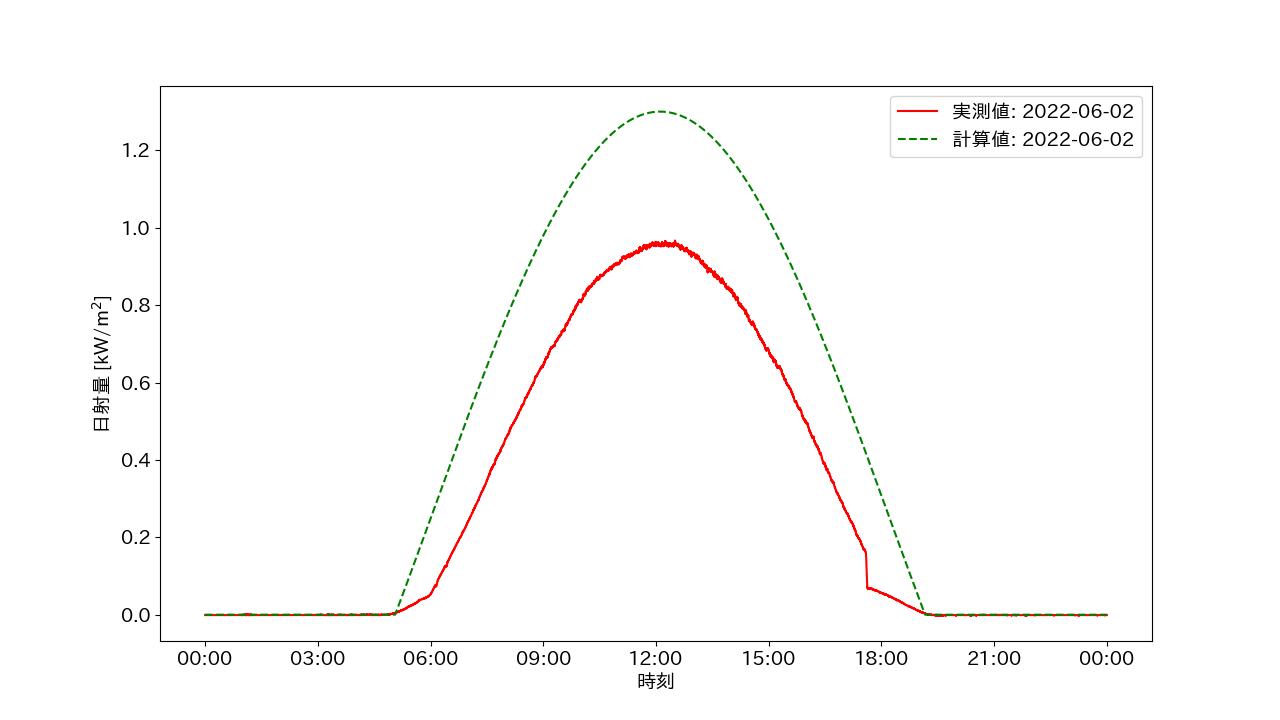
\includegraphics[width=160mm]{sotu/figure/2/original-20220602-corr.png}
    \caption{2022年6月2日の日射量の実測データと計算データをプロットしたもの}
    \label{20220529-p1}
  \end{center}
\end{figure}

% 20220620

\section{相互相関によるずれ時間の特定}
今回, 相互相関の計算に使用する実測データの範囲を, 2022年6月2日0時0分から2022年6月2日23時59分まで期間とする.

2022年6月2日を選定した理由として, 図\ref{20220529-p1}より, 2022年6月2日の実測データの概形は計算データの概形と類似していたためである.

実測データの計測日時の情報をもとに, 計算データを求め, これらの値を入力として相互相関を計算する.

相互相関の計算結果より, 計算値の日時を実測値より124秒進めた際に, 相互相関の値が最大となった.

しかし, 今回使用した実測データには計測日時のずれは殆どないため, 計算データの日時を進めていない際に実測データとの相関が最大となるのが正しい.

これは, 日射量の計算式の予測精度が低いことが原因であると考えられる.

\section{日射量の計算値の予測精度改善}

日射量の計算値の予測精度を改善するため, 式(2.1)~式(2.7)を使った方法ではなく, pvlibというライブラリを使用して, 任意の緯度経度と日時における日射量を求めて相互相関を計算する.

\section{pvlibの概要}
pvlibは, 太陽光発電システムの性能シミュレーションや関連するタスクを実行するための関数とクラスのセットを提供する, コミュニティが開発したツールボックスである. 

以下は, pvlibの主な特徴である.

\begin{itemize}
  \item 太陽位置計算: pvlibは, 地球上の任意の場所における太陽の位置を計算する機能を提供する. これは, 太陽の方位角や高度角を求めるのに使用される. 
  \item 大気透過モデル: 大気を通過する太陽放射の量や質を推定するモデルが含まれている. 
  \item 太陽光発電システムの性能モデリング: 太陽光発電モジュールやインバーターの性能モデルが含まれており, 異なる条件下での太陽光発電システムの出力をシミュレートできる. 
\end{itemize}

\section{実測値とpvlibを使って求めた計算値の比較}
Elasticsearchサーバーから取得した日射量データと, pblivを用いて求めた日射量データをプロットしたものを図\ref{2-p1}に示す.
図\ref{2-p1}はElasticsearchサーバーから取得した2022年6月2日の日射量データと, リサイクル館の緯度経度と日付情報を入力としてpvlibより求めた日射量の計算値をプロットしている.

図\ref{20220529-p1}と比較して, pvlibより求めた日射量が実測データにより近い概形となっていることが分かる.

\begin{figure}[h]
  \begin{center}
    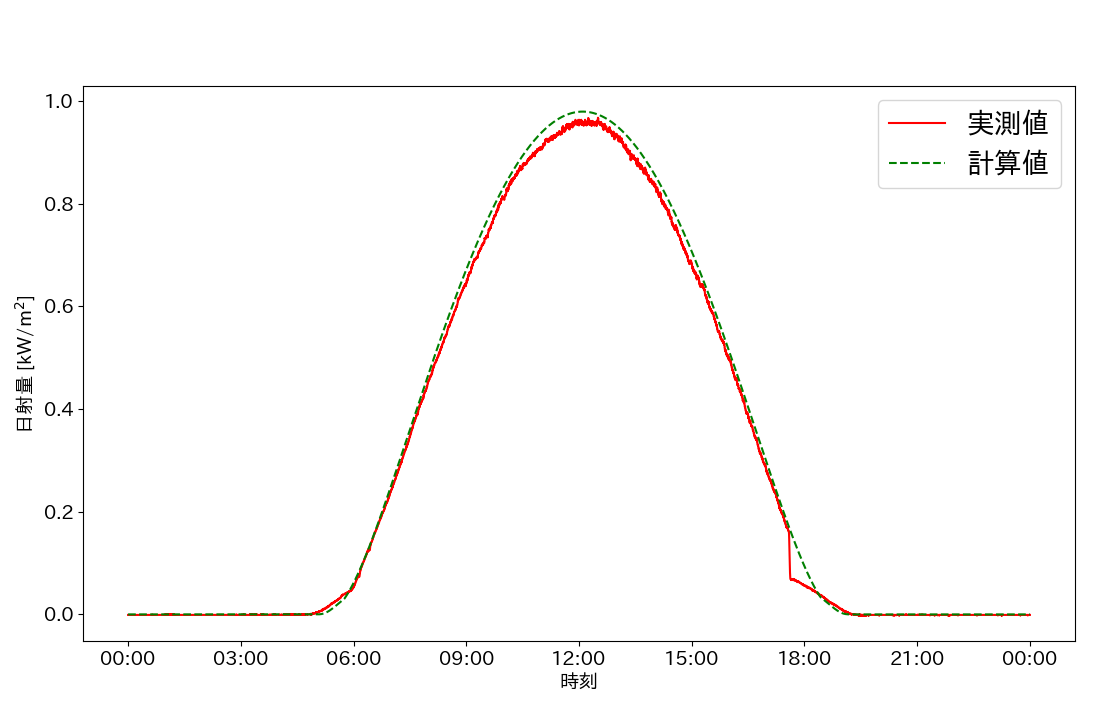
\includegraphics[width=160mm]{sotu/figure/2/pvlib-20220602-corr.png}
    \caption{2022年6月2日の日射量の実測値と計算値をプロットしたもの}
    \label{2-p1}
  \end{center}
\end{figure}

\section{pvlibを用いて計算した日射量を使用した, 相互相関によるずれ時間の特定}
相互相関の計算に使用する実測データの範囲を, 2022年6月2日0時0分から2022年6月2日23時59分まで期間とする.

実測データの計測日時の情報をもとに, pvlibより計算データを求め, これらの値を入力として相互相関を計算する.

相互相関を求めた結果, 計算値の日時を実測値より74秒進めた際に, 相互相関の値が最大となることが分かった.

式(2.1)~式(2.7)を用いて求めた日射量データ用いて相互相関を計算した時と比較して, 124秒から74秒へと50秒改善した.

\section{結言}
本章では太陽光発電の計測データの補正について述べた. 
次章では学内ゾーンで稼働している Elasticsearch クラスタへのデータ移行について述べる. 